\ifdefined\included
\else
\setcounter{chapter}{3} %% Numéro du chapitre précédent ;)
\dominitoc
\faketableofcontents
\fi

\chapter{Modeling and Planning for Concurrent and Compliant Joint Action Execution}
\chaptermark{Concurrent and Compliant Joint Action Execution}
\label{chap:4}
\minitoc

\chapabstract{This chapter presents my second main contribution, proposing a new human-aware task planning approach based on a step-based model of compliant and concurrent joint action. The approach's description is supported by empirical results proving its effectiveness in terms of the latitude of choice given to the human and the satisfaction of their internal preferences. We further validated this by developing an interactive simulator used for a user study, described in the following chapters.}

\section{Introduction}

\textit{From HRI paper}

In the context of \acrshort{hrc} for a shared task~\cite{selvaggio2021autonomy}, we believe, based on the literature on joint action~\cite{sebanz_2006joint,sebanz-2009,clodic-2017,gordon-2023}, that the key towards a seamless interaction is, to consider the human as an uncontrollable agent and to be fully and concurrently compliant with them. 
The human should not be dictated which action they must perform, as in~\cite{roncone2017transparent,buisan_hatpehda_icra}, and the robot must comply with possible human decisions and actions during execution.

To collaborate with such humans with their (hidden) preferences, one can devise an online planning scheme coupled with a plan executor. 
However, in order to maintain real-time performance, online planning generally keeps a restricted horizon. 
Therefore, decisions taken online may lead to a dead end or may not lead to an optimal solution. 
Offline planning overcomes these issues. 

We propose a new \textit{offline} task planner which extends an existing human-aware planning system addressed in~\cite{buisan_hatpehda_icra}. 
The new planner is designed to take into account a \textit{Model of Execution}, which is in the form of an automaton and mainly inspired by the joint actions schemes. 
The model captures humans' latitude in their decisions. 
The planner's output is the robot's behavioral policy, which describes the robot's action in a state such that the action is congruent and compliant with the human's decision in this state and their (estimated) preferences and that it is also legal to be executed in parallel. 
Our framework also allows humans to share their (new) preferences at any time during execution while the robot's policy is adapted online to that. 
In addition, our approach considers social signals to enhance execution by minimizing uncertainties. Both humans and robots issue signals to clarify situations such as performing an action, waiting for the other agent's necessary actions, or indicating a desire to remain passive.

In this chapter, we discuss relevant related work before describing the joint action model of execution that is central to our approach. 
We then describe the task planning problem and then introduce our novel framework. 
The following two sections to that, explain how the robot policy is generated by a three-step process: \textit{exploration}, \textit{characterization}, and \textit{generation}. 
We empirically evaluated our approach in simulation. With a BlocksWorld scenario, we show how our approach can effectively produce a concurrent robot behavior that is compliant with human online decisions and preferences.  

\section{Related works}

There have been a few attempts to cater to concurrent execution, but they deal with explicit time to manage concurrency~\cite{CirilloKS09a,kockemann2014grandpa}. 
In~\cite{CirilloKS09}, the robot does not plan actions for humans but forecasts their actions/plans from their activities and bases its own decision on the distribution of possible human plans. Here, robots can perform actions concurrently, carefully estimating/managing the completion time of the agents' actions. 
We can see the human activity recognition part as a form of our \acrfull{id} process of the automaton used. The robot needs such a plan/goal recognition technique to be compliant with the human's decisions. 
But, unlike ours, they do not consider an explicit shared goal among the agents. Hence, humans are not concerned with stuff robots might be interested in during collaboration, e.g., giving signals to be passive. 
We believe that a shared goal creates a different context in \acrshort{hrc} than the robot just being compliant with an estimated human's goals/plans. 
Moreover, we claim that dealing with concurrent actions is inevitable in planning, even if actions are instantaneous, to effectively deal with multiple agent systems~\cite{CrosbyJR14,ShekharB20}, especially if a human operator is involved, like in our case. 
We extend HATP/EHDA~\cite{buisan_hatpehda_icra} to demonstrate that.

In another work, both \textit{recognition} and \textit{adaptation} take place simultaneously and comprehensively~\cite{levine2014concurrent}. 
It deals with the action scheduling of an already generated contingent plan comprising human and robot actions. 
It outputs schedules for the robot actions that can execute concurrently, but to do that, explicit temporal constraints are considered. 

Ramachandruni, Kent, and Chernova (2023)~\cite{RAMACHANDRUNI2023} propose a communication-free human-robot collaborative approach for an adaptive execution of multi-step tasks. 
In their approach, the robot observes and supports human decisions, actively selecting actions to optimize collaborative task efficiency. 
Unlike our approach, they introduce an extended collaborative HTN representation with role assignment for planning and state tracking during execution, which is more in line with~\cite{roncone2017transparent}. 
In contrast, we employ two distinct HTNs for robot and human capabilities and use an AND/OR tree for exploration and execution tracking. While their online planning may enhance scalability, optimality is not guaranteed. 
Also, our scheme accommodates both verbal and non-verbal communication, allowing the human to express preferences that update the robot policy online. 

\section{Joint Action Model for Planning}

    \subsection{Rationale and Example}



Our task planning approach uses a model of execution to improve the fluency and amenability of \acrshort{hrc}. 
This model is in the form of an execution controller and is based on several key notions and mechanisms borrowed from studies on joint actions~\cite{Sebanz_2016,kourtis2014attention}, and adapted to Human-Robot Joint Action~\cite{clodic-2017,curioni-2019}.
The key idea is that co-acting agents co-represent the shared task context and integrate task components of their co-actors into their own task representation~\cite{Schmitz-2017, Yamaguchi-19}. Also, coordination and role distribution rely strongly on reciprocal information flow, e.g., social signals~\cite{curioni-2019}, prediction of other's next action~\cite{luke-2018}.

Our proposed execution model is implemented on a robot that co-acts with a human, integrating explicit representation and exploration of the task representations for the robot and for the human. 
It also identifies precisely how reciprocal information flow is used in task execution (detecting and interpreting human actions, signals produced by the robot while acting, and also when the robot waits for human actions or their signals).

Another essential question is the criteria for choosing the next action, or more globally, how to share the load between the two co-actors. The choice depends on the context and actors' preferences~\cite{Gombolay-2015, Strachan-2020, Curioni-2022}. 
Concerning the case when one actor is a robot, we think it is important to provide a standard default behavior of the robot where the robot does its best to reduce human load but still leaves full latitude to act whenever humans want. 
Our scheme provides this ability and also allows humans to inform about their preferences at any moment.

\begin{figure}
    \center
    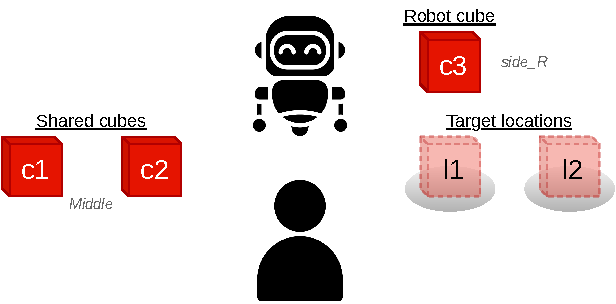
\includegraphics{Chapter4/example_conflict_pick.pdf}
    \caption{Example of conflict for a concurrent joint action. 
    Shared cubes, \emph{c1} and \emph{c2}, can be picked up by both agents, and only the robot can pick \emph{c3}. 
    Agents can simultaneously pick up both shared cubes but must coordinate their actions. Otherwise, they might conflictingly try to pick the same cube. 
    Similarly, another coordination is required to avoid placement conflicts between locations \emph{l1} and \emph{l2}.
    However, notice that the robot can pick \emph{c3} without any risk of conflicts with the human action.}
    \label{fig:conflict_pick}
\end{figure}

To better understand the problem we are trying to solve, let's consider an example where concurrent agent's actions can be conflicting. This example consisting in a simple pick and place task is depicted in fig~\ref{fig:conflict_pick}. The human and the robot have to pick cubes, \emph{c1} and \emph{c2}, that both can reach. 
The cubes can be picked up simultaneously unless the agents try to pick the same cube, which causes conflicts between their actions. As a result, despite being executable in parallel, the actions are interdependent. Thus, the agents must coordinate their actions for a smooth execution.
A similar coordination must happen when placing the cubes to avoid conflicts between \emph{l1} and \emph{l2}.
However, a third cube \emph{c3} is present and can only be picked up by the robot. The robot can pick \emph{c3} without any risk of conflicts with the human action. 

This example illustrates the need for coordination even for simple tasks. It also shows that considering possible conflicts can also be a criterion for optimizing. Thus, the best robot action might be to pick up \emph{c3} instead of one of the shared cubes to avoid potential conflicts, even if \emph{c3} is more distant and more costly to pick than \emph{c1} and \emph{c2}.
This example also highlights the relevance of exploring several possible executions of concurrent actions while planning to anticipate and evaluate such situations and produce a robust, compliant, and efficient robot policy. This is why, based on joint action literature, we formulated a model of concurrent joint action execution described below that will guide our planning search.

\subsection{Abstracted Joint Action Model for Planning}

\begin{figure}
    \centering
    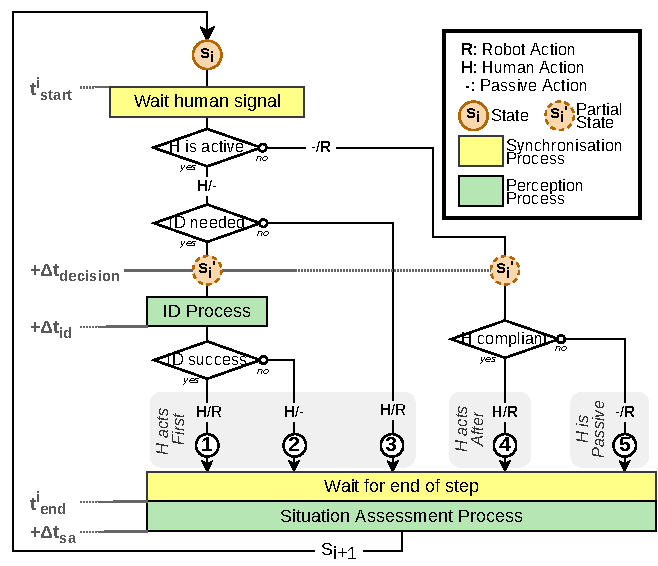
\includegraphics[width=0.8\linewidth]{Chapter4/simplified_automaton.pdf}
    \caption{
    Abstracted Model of Execution in the form of an automaton run by the robot. It captures the latitude of uncontrollable humans in their actions and guides our task-planning approach.
    In this paradigm, the two agents can act concurrently, but one always complies with the other's decision.
    Here, humans are always free to decide whether to start acting first, after the robot, or not to act at all.
    To be compliant, the robot attempts to identify human decisions using perception and situation assessment as well as possible collaborative human signaling acts (e.g., gestures or speech).
    }
    \label{fig:simplified_model_exec}
\end{figure}

% Full page figure formats w/r line of caption:
% - 5 lines = 210x294 ratio
% - 4 lines = 210x301 ratio
% - 3 lines = 210x308 ratio

The model of execution we formulated, depicted in fig~\ref{fig:simplified_model_exec}, is inspired by joint action literature and describe the agent's coordination during execution. It comprises synchronization and perception processes based on social signals exchanged between the agents, such as starting an action (arm motion), hand gestures, or verbal communication. This section presents a simplified and abstract version of this model that suffices to guide our planning framework. A complete version that explicitly models the human behavior and exchanged signals is provided in the next chapter and used to supervise the execution of the produced robot policy.  


% \textbf{TODO: add numbered marks in the figure to refer to easily for description, also describe the conditions: H is active, etc...}

The model describes the possible transitions from a given state to another, step by step. The robot always informs the human about the beginning of a step and then waits for their decision by looking at social cues. The top yellow rectangle in the figure represents this waiting process. This human decision can either be to start acting or to be passive. Hence, the robot always lets humans first decide which action they want to perform, including the choice to be passive. This decision is detected with perception by tracking social cues such as human motions and hand gestures.

The diamond shapes below the first synchronization process are conditions, driving the automaton into different branches depending on specific conditions. First, we differentiate between cases where the human is passive and cases where the human is active (``H is active''). 
When the human is performing an action, the `yes' branch, we first check if the human action must be identified or not. So far, only the fact that the human is acting is known, but not yet which particular action they are performing. 
To avoid potential conflicts, we consider that there is no need to identify the human's action if the best robot action does not depend on the human decision. For instance, consider in the cube picking example presented in figure \ref{fig:conflict_pick} that the cube \emph{c3} is easier to pick and place for the robot than the two other one. Thus, regardless of which cube the human picks, the robot should pick \emph{c3}. Its best action does not depend on the human decision, and there is no need to identify the human's action. However, if \emph{c3} is effectively harder to place than \emph{c1} and \emph{c2}, the robot must first identify which cube the human is grabbing to pick the other one. As a result, the model differentiates the cases where the human action must be identified (``ID needed'') or not. If not, then the robot can directly start acting (branch 3). Otherwise, the \acrfull{id} process is executed and may either be successful (``ID success'') or not. If not, to avoid any potential conflict, we decided that the robot should remain passive (branch 2). If the human action has been successfully identified, the robot can perform the best corresponding action concurrently (branch 1).

In the case where the human decided to be passive, the robot should start acting. 
However, while the robot is acting, we consider that the human is free to either remain passive until the next step (branch 5) or to ``change their mind'' and start acting (branch 4).
This is represented by the diamond shape ``H compliant''. When the human decides to start acting after the robot starts, the human can only perform actions that do not conflict with the already started robot action. Note that this case can be seen as a way for the human to let the robot decide and then comply with the robot's decision. Still, the human decided to let the robot decide, thus, the human is given as much latitude of choice as possible.

Overall, at every step of the execution, the human is free to decide: 1) to start performing any feasible action, the robot will comply with this decision; 2) to let the robot decide and act first, and then purposely we compliant with the robot; 3) to be passive and let the robot act alone.

When both agents finish their actions, the step is considered as \textit{``over''}. This synchronization is represented by the bottom yellow rectangle ``Wait for end of step''. Then, a Situation Assessment Process is executed to assess the new world state ($s_{i+1}$), which is the result of the concurrent actions being executed in the state $s_i$. Once the next state is identified, the automaton repeats until the task is solved and a goal state is reached.

Note that if, for any reason, both agents are passive during a step, the state is unchanged so the step is repeated. 

%%%%%%%%%%%%%%%%%%%%%%

% Let's describe this simplified model in the form of an automaton on which on planning algorithm is based on.
% In a state, a human decision can result in one of three outcomes.
% First, the human can choose to act first (\textit{left~subtree}).
% If the robot's best action is not in conflict with the human action (e.g., \textit{pick~C}), the robot can safely perform this action concurrently with the human operator (\textit{branch~3}).
% However, if the robot's best action is either \textit{pick~A} or \textit{pick~B}, the human action must be identified first with a subroutine in order to be compliant with it.
% If this subroutine is successful the robot can perform any action which is congruent with the identified human action (\textit{branch~1}). 
% This includes the robot's choice to be \textit{passive} and let the human act alone. 
% However, if the robot is unable to identify the human action, it must remain passive in order to avoid potential conflicts (\textit{branch~2}). 
% Then, the human can either decide to be \textit{passive} or to act after the robot (\textit{right~subtree}). 
% In both cases, the human is \textit{passive} at the beginning, making the robot to start performing alone a feasible action. 
% While the robot is acting, the human is free to remain \textit{passive} until the next step (\textit{branch~5}) or to choose a congruent action to act concurrently (\textit{branch~4}). 
% As a result, the human can always choose to 1) act first, 2) act after the robot, or 3) not act at all. 
% The robot will always be compliant with these online human decisions.

% When both agents finish their actions, the step is considered as \textit{``over''}. 
% Then, another subroutine assesses the new world state ($s_{i+1}$), which is the result of the concurrent actions being executed in the state $s_i$, before repeating the whole process until the task is solved.

% Note that if both agents are passive (the human decides to be passive when the robot cannot act) then the step is repeated. 

\section{Problem and Solution Specifications}

Compared with the original HATP/EHDA specifications, this contribution slightly modifies the problem and solution specifications. This section describes the main differences.

    \subsection*{Problem Specification}

Belief divergences are out of the scope of this particular work. Hence, for simplicity reasons, we consider the two beliefs (robot and estimated human ones) as always aligned, and they are represented as a unique world state. However, we are convinced that this work could be adapted easily to consider the two distinct beliefs.

The problem is specified as shown here \ref{sec:problem_spec} in Chapter~\ref{chap:2}. For simplification purposes, in this contribution, no belief divergence is considered. Therefore, unlike Chapter~\ref{chap:3}, the two agents beliefs are always aligned and initialized with a same initial world state using state variables. Then, distinct human and robot action models are described with HTNs and distinct human and robot initial agendas are provided comprising a shared task to accomplish. 

\subsection*{Solution Description}

\begin{figure}[h]
    \centering
    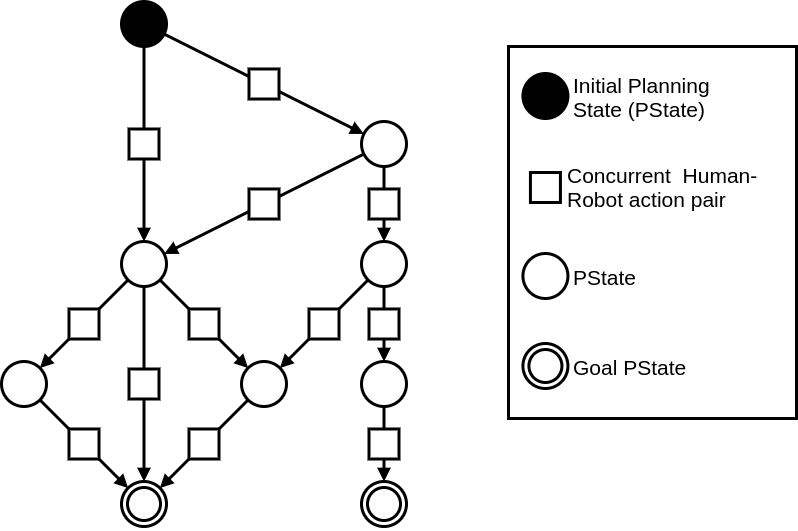
\includegraphics[width=0.7\linewidth]{Chapter4/solution_graph.png}
    \caption{Directed acyclic solution graph}
    \label{fig:solution_graph}
\end{figure}

A Planning state, referred to as p-state, corresponds to a state in which the planning problem is while progressing toward a solution. It corresponds to the definition of a \textit{state} from Chapter~\ref{chap:2}. A p-state contains the current world state (aligned beliefs of the agents) and the respective agenda of the human and the robot. Thus, keep in mind that p-states are very different from world states.
The initial p-state is formed using the initial human-robot agendas and the initial world state given in the problem specification. P-states are connected through pairs of concurrent human-robot actions. Note that we consider passive actions, hence, there may be only one active agent in a pair if concurrent human-robot actions. A goal p-state is characterized by a world state satisfying given goal conditions and by empty agendas.
The exploration produces a \acrfull{dag}, referred as the search graph, from the initial p-state to several goal p-states through sequences of concurrent action pairs. Thus, any path from the root to a leaf is a possible plan. Once the exploration done, search graph computed, another process extract the optimal robot policy from the graph. In the manner of an AND-OR tree, this policy indicates for all p-states the best concurrent robot action (OR node) to execute to be compliant with any possible human action (AND node).


First, we provide a few clarifications about the \acrshort{dag}. Nodes represent p-states and are connected with each other through directed edges representing human-robot concurrent action pairs. The graph has one root node (with no parent) which is the initial p-state. All leaf nodes (with no children) represent goal p-states. 

It is one of our design choices to do not consider explicit action costs and perform an exhaustive offline search to produce this search graph in order to solve a problem. Since the policy generation is rapid it allows generating and updating the robot policy online according to human feedback. 


\begin{figure}
    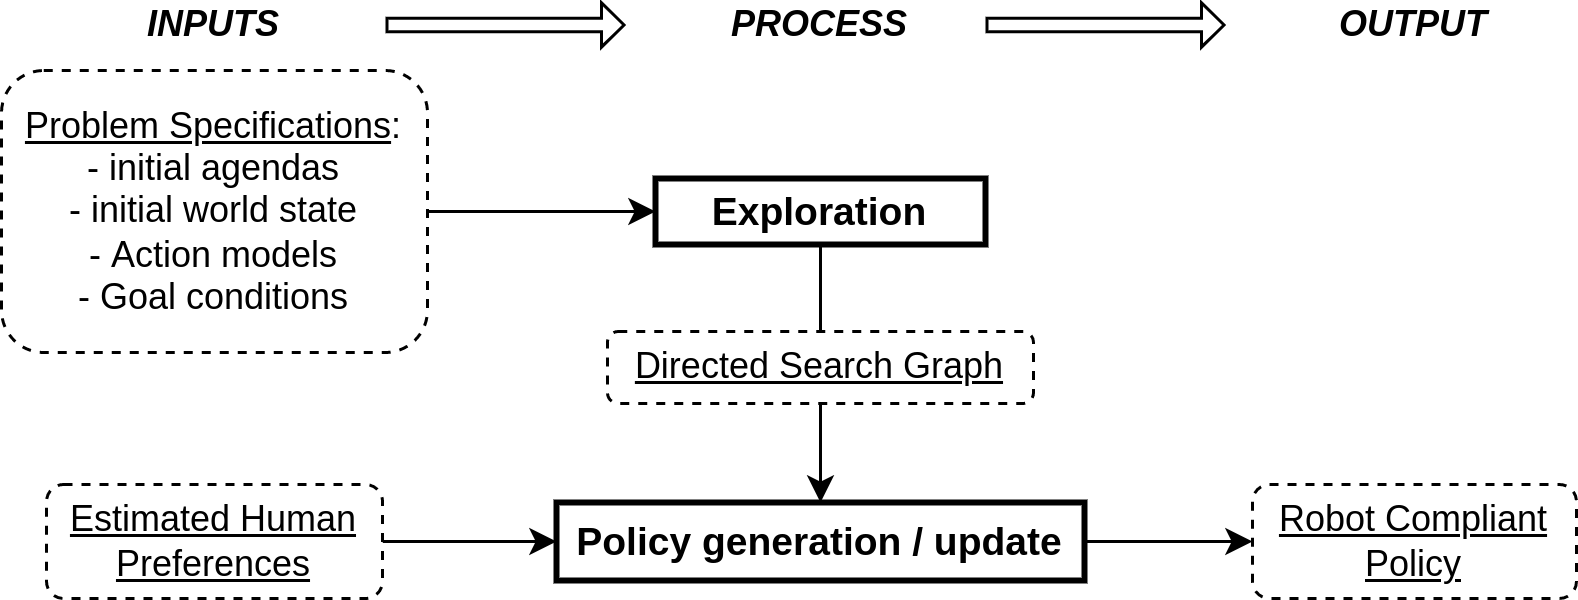
\includegraphics[width=\linewidth]{Chapter4/overall_process.png}
    \caption{Overall planning process}
    \label{fig:overall_process}
\end{figure}

\section{Exploration and Search Phase}

This section details how the exploration happens and thus, how the search graph is generated. This requires several sub-process, which are each detailed here. First, the overall exploration process is presented, and next subsections provide details on the sub-processes mentioned in the overall process.

    \subsection{Overall Exploration Process}

We keep track of the p-state to explore, and this set is being initialized with the initial p-state. Then, until the set is empty, we select one and explore it.
First, from this selected p-state, every possible concurrent human-robot action pairs are computed considering both agendas, the world state and reasoning on the compatibility of the actions in terms of preconditions and effects. This process requires several sub-steps and is detailed later. Thus, we obtain several action pairs leading to the same amount of new p-states (with updated world states and agendas).
Second, we check if any of the newly created p-state are similar to any existing p-state. If so, we can "merge" them to avoid redundant computations. To do so, we basically keep track of the unique p-state already checked and for each new p-state we check if it is similar to one of the already checked one. 
If not, the new p-state is added to the set of already checked p-states. 
If a similar one is found, the new p-state is deleted, and the action pair leading to it is connected to the existing p-state instead.
Eventually, the remaining new p-states are added to the set of p-states to explore. 
The exploration is over when the set of p-states to explore is empty. The obtained \acrshort{dag} corresponds to the "search graph" where any path from the initial p-state to a leaf corresponds to a possible execution trace.

    \subsection{Compute Next Agent Actions}

From a p-state, more precisely from a world state and an agenda, we can estimate the next actions an agent is likely to perform. Doing so is referred to as the refinement process. We use the corresponding action model in the form of a \acrfull{htn}. Here, the agendas are considered as lists of abstract or primitive tasks, where primitive tasks can be executed (actions), and abstract ones must be decomposed into several other subtasks. 
The refinement process consists of applying applicable methods of the first task of the agenda until it is primitive. When several methods are applicable, they are all applied in a distinct refinement trace.
Eventually, for each different sequence of applied methods, we obtain a new agenda starting with a primitive task. For each such primitive task, we create a copy of the world state contained in the given p-state, and we apply the corresponding action, updating the world state. 
Finally, for each possible action, a new p-state is created with the refined agent agenda, the unchanged other's agenda, and the updated world state. 
Note that this process can ``generate'' default passive actions in several cases. First, when an agent's agenda is empty, an \textit{IDLE} passive action is inserted as the first primitive task in the agenda. This means that the agent has nothing to do and, thus is likely to remain passive. When there are no applicable methods or when the primitive task is not applicable, then a \textit{WAIT} passive action is inserted. This means that the agent still has something to do but cannot do it. Note that when computing the concurrent pairs of action, we also add the \textit{PASS} action, which corresponds to the agent being voluntary passive, despite having something to do. Note also that these different passive action types help to understand the generated plans better, but they are treated similarly in the planning process.

    \subsection{Concurrent Action Pairs Computation}

This sub-process computes from a given p-state all possible concurrent action pairs that may be executed. It is based on the previously described refinement process. The main objective of this sub-process is to identify the next actions the agents are likely to perform to reach the goal and identify which of them can be executed in parallel. The classical way to do such reasoning is by analyzing the preconditions and effects of the two actions and determining if there are conflicts between them, e.g., the effects of the first action make the preconditions of the other false.
However, our current python implementation of the planner is convenient but has no ``explicit'' preconditions and effects. Everything is defined through python function. The effects of an action are a function with a world state as input which returns the updated world state. Action preconditions are functions with a world state as input and return a boolean. Methods are functions with world state as input and return a list of tasks to update the agenda with. Methods also have preconditions working similarly than action preconditions. 
Hence, extracting the explicit effects and preconditions of an action is challenging. That is why we decided to rely on an assumption to check the compatibility of concurrent actions. 
Consider two actions $A$ and $B$ tha can be sequentially performed in both orders, i.e., $A \rightarrow B$ and $B \rightarrow A$. Then, we assume that there are no causal links between the two actions and that they can be performed concurrently. The only care to take is shared resources such as a tool that would only be used during the action, making it available before and after but not during the action. To tackle this issue, shared resources are explicitly declared in the world state and in the action models. Two actions requiring the same shared resource cannot be parallelized.
Such approach to check if two actions are mutually exclusive and if they can be parallized comes with a benefit. Indeed, it only needs an action precondition boolean function. As a result, actions estimations can be a black box with only basic low level actions preconditions descriptions. This way, we can easily replace the way we estimate the next actions each agent is likely to perform. Especially for the human, we could use a pretrained human activity estimator neural network or more classical planner like PDDL. 

With the causal principle above in mind, we proceed as follows to compute the possible concurrent action pairs from a given p-state. We start by estimating all possible human actions by refining the human agenda generating a new p-state for each possible action. For each such p-state, we first create an action pair where the robot is passive by inserting a \textit{PASS} robot action. This \textit{PASS} pair is stored among all other `human pass pairs''. Second, we refine the robot agenda to obtain all feasible sequences of human then robot actions and their associated p-states. We refer to them as the sequential human starting pairs. Symmetrically, we compute the sequential robot starting pairs and "robot pass pairs" by starting with the robot and then refining the human agenda.

Eventually, every action pair which is present in both the human and robot starting pairs is extracted and added to a set of concurrent action pairs. 
Additionally, here, passive actions are always parallelizable with another regular action. The only case where this could not be the case is when considering ``joint actions'' requiring the two agents to lift a object together. For now, such actions are not considered. Thus, the two sets of \textit{PASS} pairs are directly added to the set of concurrent action pairs. 
Lastly, a double passive pair with two PASS is generated and added to the concurrent set. This pair is special since it does not update the world nor the agendas. Hence, it leads back to the previous p-state without progressing toward the goal. These pairs do not need to be explored and help it different ways. First, it helps the execution, for instance, when only the human can act but decides to pass voluntarily. Then, the policy will natively stay in the same p-state. Second, it is easy to detect dead-ends because they correspond to double \textit{WAIT} pairs. In such cases, both agents cannot act, and they remain stuck without solving the task.  
Last, double \textit{IDLE} pairs indicate that both agendas are empty and, thus, that the task is solved. 

The obtained set of concurrent action pairs corresponds to all possible concurrent actions that the human and the robot can execute in parallel in the initially given p-state. Each possible pair leads to a new p-state with updated agendas and world state, creating a tree structure. 

    \subsection{Merging p-states}

Although the tree structure produced by the process described above is complete and sound, it is inefficient and scales poorly. Indeed, during the exploration, we are likely to encounter similar p-states several times. For instance, consider an action pair where both the human and robot are active, leading to a new p-state. Now, consider an action pair where only the human is active, and a second where only the robot is active. Performing those two last pairs in both orders creates two other branches. However, even though the trace is different, the three p-states are identical (same world state and agendas), and it's highly redundant to explore independently each of them. That is why, after each computation of the concurrent action pairs, we check if any of the newly generated p-state is similar to an existing one. If so, we connect the corresponding pair to the existing p-state to avoid redundant explorations. Doing so, we transform the tree structure present in the previous chapters into a \acrfull{dag} (on the condition that we do not consider double \textit{PASS} cycles). In the manner of a tree, we will refer to nodes without children as leaves nodes, which are goal p-states. Hence, now, each leaf can be reached with several paths. 
When looking for similar existing p-state, we assume that p-states which are parent with the new p-state, directly of not, will necessarily be different, and thus they are excluded. This speeds up the comparison process. 

Note also that for the p-states to be similar despite different concurrent executions like explained just above, we had to remove the \textit{partial plan} present in specification described in Chapter~\ref{chap:2}. To significantly improve the performance and use the \acrshort{dag}, we can no longer reason on the \textit{partial plan} of the agents. However, we can still define a dedicated state variable to keep track of specific events or action sequence if it influences the task decompositions. For instance, it would be relevant to define a state variable to keep track of how many times the robot requested punctual human help like in the example of Chapter~\ref{chap:2}.    

\section{The Robot Policy}

First of all, as depicted in figure~\ref{fig:and_or}, all child concurrent action pairs of a p-state ($PS / ps_i$) can actually be seen as an AND-OR graph. Since we want to preserve the latitude of choice the human has at execution, each possible human choice of action is considered as an AND edge and leads to a partial p-state ($PS' / ps_i^j$). From a partial p-state, each compliant concurrent robot action is considered as an OR edge and leads to another p-state.

Notations: A p-state is referred to as $ps$, and $ps_i$ is the $i$-th p-state. A partial p-state is referred to as $ps'$, and $ps_i^j$ is the $j$-th partial p-state of the $i$-th p-state.

Thus, generating the robot policy $\Pi$ consists of identifying the best concurrent compliant robot action $RA^*$ for each possible human action or partial p-state $ps_i^j$.

These best concurrent robot actions are determined by aiming to optimally satisfy an estimation of the human preferences regarding the task. Eventually, at execution, the human is free to perform any of the explored actions and the robot will accordingly perform an optimal concurrent action to both solve the task and satisfy their estimated preferences.

Hence, before giving more details about the policy itself, we first describe the format of human preferences, how we could estimate them, and what it allows us to do. After, we describe the actual process to generate the robot policy from the search graph using the estimated human preferences


% **The robot policy consist in performing the best robot action according to the node and the human action, i.e., robot action stored in the "best compliant" pair corresponding to the human action.
% If all "best compliant" pair have the same robot action, the robot can perform as soon as the step stars, otherwise the human action must be identified.**

\begin{figure}
    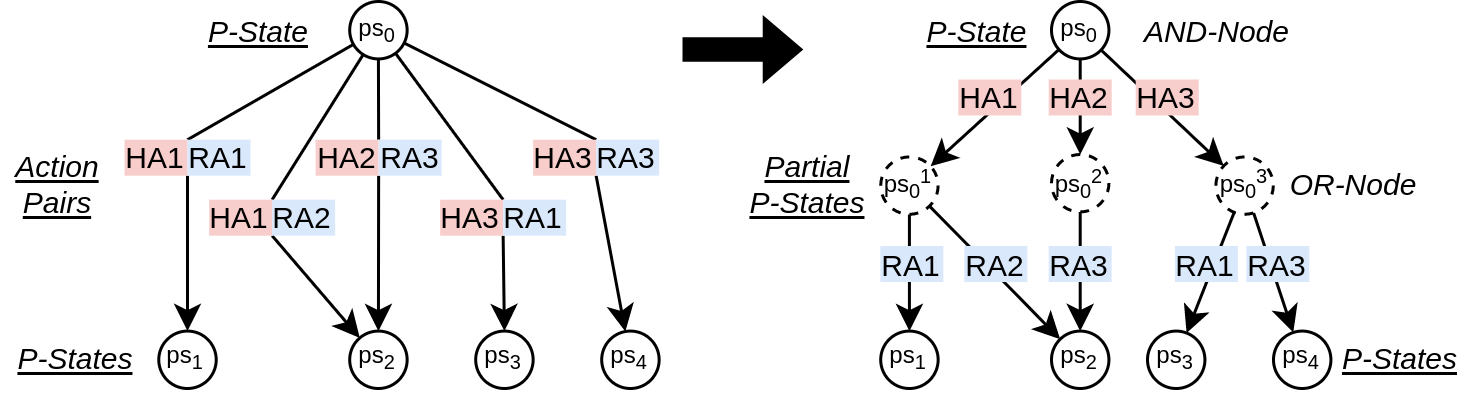
\includegraphics[width=\linewidth]{Chapter4/and_or_tree.png}
    \caption{AND-OR graph representation of the action pairs. 
    The robot policy must be compliant to any decision of the human. Hence, the problem can be seen as an AND-OR graph where, for each possible human choice of action (AND node), we must determine the best concurrent robot action among the possible robot actions (OR node).
    }
    \label{fig:and_or}
\end{figure}


    \subsection{Using Estimated Human Preferences for Plan Evaluation}
% estimations, format, Discussion(often inaccurate, hence our Approach), consider metrics, is a prioritized sequence of metrics to max or min, allow comparison of metrics

In this approach, instead of trying to minimize action and social costs, which are challenging to estimate accurately and quantitatively, we aimed to satisfy an estimation of the human preferences. In a way, the costs are reflected in the human preferences. Our approach is to characterize each possible trace with a set of various metrics such as follows:

\begin{itemize}
    \item \textbf{Time of Task Completion}: Time step at which the task if achieved.
    \item \textbf{Time of End of Human Duty}: Time step after which the human can remain passive.
    \item \textbf{Human Effort}: Number of non-passive human action.
    \item \textbf{Global Effort}: Number of non-passive human and robot action.
    \item \textbf{*Passive While Holding}: Number of steps where an agent is passive while holding a cube.
    \item \textbf{*Number of Drops}: Number of times an agent drops a cube (place back a cube on the table, not in the stack).
\end{itemize}

Note that general metrics are complemented with additional domain-specific metrics (marked with a star *), as given in the problem specification. The set of metrics helps to characterize and evaluate each possible trace. However, even if the possible plans are characterized, we so far have no way to compare them and find the best one. Doing so requires additional criteria indicating how to prioritize and compare the different metrics.

The preferences can be estimated, given verbally or by any other means. Here, we consider the human preferences in the following form. These preferences are an ordered list of the metrics characterizing the traces. Note that all metrics in the list above do not need to be present. This ordered list indicates if each metric should be maximized or minimized and with which priority. For instance, assuming the preferences aim to minimize all metrics, the plan with the lowest first metrict of the list will be considered as better. If the plans have an equal first metric, then we use the second metric, and so on. Here are two arbitrary examples of human preferences trying respectively to finish the task as fast as possible ($preferences\_1$) and to minimize the human effort ($preferences\_2$) (all metrics are minimized):

\begin{equation*}
    preferences\_1: TTC > GE > HE > TEH > PWH > ND 
\end{equation*}
\begin{equation*}
    preferences\_2: HE > TEH > TTC > GE > PWH > ND 
\end{equation*}


Note that estimating either human preferences or explicit action and social costs is challenging and is hardly accurate. Those are very context-dependent and can even vary over time.
Being aware of this, we use the estimated human preferences as a guide for the robot behavior. However, we also make sure to comply with the human activity to lessen the impact of erroneous estimations. 

    \subsection{Generation}

\begin{figure}
    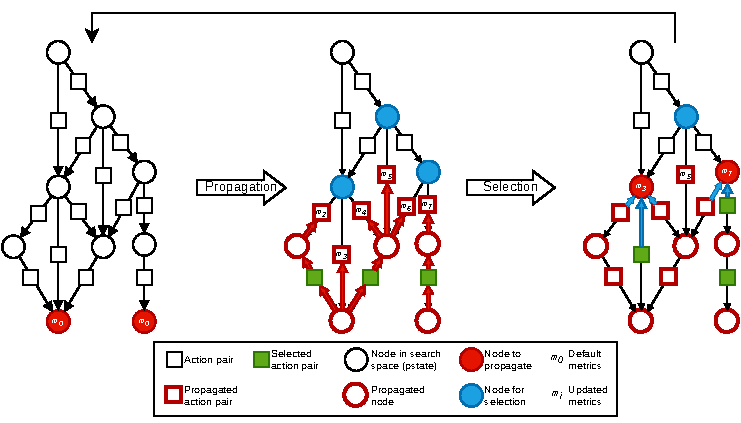
\includegraphics[width=\linewidth]{Chapter4/policy_generation.pdf}
    \caption{Policy generation process illustration on an arbitrary search graph. Propagation and Merge processes repeat until there are no more p-state/node to propagate or for selection.}
    \label{fig:policy_generation}
\end{figure}

To generate the robot policy $\Pi$ from the search graph, we proceed from the leaves to the root. 
Overall, we progressively compute the set of metrics for each possible trace. When reaching a p-state with several children, we compare the metrics of the different traces leading to this node. We can then identify the best trace leading to each partial p-state and the best trace leading to the p-state. Each best trace to a partial p-state is used to update the robot policy, and the overall best trace is used to continue the propagation with the best reachable set of metrics.
This process is achieved by repeating two sub-routines detailed just below, namely \textit{Propagation} and \textit{Selection}. 

\begin{algorithm}
\caption{Policy Generation}\label{alg:policy_generation}
\begin{algorithmic}[1]

\State \textbf{input}: $leafNodes$ \Comment{Set of all leaf p-states from the search graph}
\State $psToPropagate \gets \emptyset$
\State $psForSelection \gets \emptyset$

\State $Initialization(psToPropagate, leafNodes)$

\While{ $psToPropagate \neq \emptyset$ and $psForSelection \neq \emptyset$ }
    \State $Propagation(psToPropagate, psForSelection)$
    \State $Selection(psToPropagate, psForSelection)$
\EndWhile

\end{algorithmic}
\end{algorithm}

    \subsubsection{Format and Initialization}

During this process we compute and store the best reachable set of metrics alternatively in the p-states and in the action pairs. Initially, we store default null metrics in every leaf p-state. Then, we keep track of two types of nodes. First, keep track of the nodes whose metrics should be propagated in the next step, stored in the set $\{psToPropagate\}$. This set is initialized with all leaf p-state nodes. The Selection sub-routine later populates this set. Secondly, we keep track of the nodes that should select among several the best set of metrics and, thus, the best actions to perform. This set is $\{psForSelection\}$ and is populated by the propagation sub-routine while being emptied by the selection sub-routine. The process is over when the two sets are empty, thus, when there are no more nodes to propagate or for selection.

% The default metrics are the following:
% \vspace{-\topsep}
% \begin{itemize}
%     \setlength\itemsep{-0.3em}
%     \item \textbf{Time of Task Completion} $= -1$
%     \item \textbf{Time of End of Human Duty} $= -1$
%     \item \textbf{Human Effort} $= 0$
%     \item \textbf{Global Effort} $= 0$
%     \item \textbf{*Passive While Holding} $= 0$
%     \item \textbf{*Number of Drop} $= 0$
% \end{itemize}

    \subsubsection{Propagation}

The propagation sub-routine is depicted in algorithm~\ref{alg:propagation} and described here. It consists of picking a node to propagate from the set $\{psToPropagate\}$. For each parent action pair of that node, we create a copy of the set of metrics of the propagated node and update the metrics according to various rules described below.
The metrics must be cumulative. 

The rules to update the standard metrics are the following (all metrics start at 0):
\vspace{-\topsep}
\begin{itemize}
    \setlength\itemsep{-0.3em}
    \item If the pair is not \textit{IDLE}-\textit{IDLE}, then \textit{Time of Task Completion} is incremented by 1.
    \item If the pair is not \textit{IDLE}-\textit{IDLE}, if the human action is passive, and if the current \textit{Human Effort} is zero, then the temporary metric \textit{Number Last Passive Human Action} is incremented by 1.
    \item \textit{Time of End of Human Duty} = \textit{Time of Task Completion} - \textit{Number Last Passive Human Action}.
    \item If human action is not passive, then \textit{Human Effort} and \textit{Global Effort} are incremented.
    \item If robot is not passive, then \textit{Global Effort} is incremented.
\end{itemize}
Rules to update domain specific metrics must be provided:
\vspace{-\topsep}
\begin{itemize}
    \setlength\itemsep{-0.3em}
    \item If human action is passive while holding a cube, then \textit{Passive While Holding} is incremented.
    \item \textit{(Similarly with the robot)}
    \item If the human action is to drop a cube back on the table, then \textit{Number of Drops} is incremented.
    \item \textit{(Similarly with the robot)}
\end{itemize}

The updated metrics are stored in their corresponding action pair. Then, two cases can occur for each parent action pair with stored metrics, referred as propagated pairs. First, if the parent node of the propagated pair has more than one child, then we add this parent node to the set $\{psForSelection\}$. Otherwise, the metrics of the action pair are stored in the parent node, which is also added in the set $\{psToPropagate\}$. 
The sub-routine repeats until the set $\{psToPropagate\}$ is empty.

\begin{algorithm}
\caption{Propagation Sub-Routine}\label{alg:propagation}
\begin{algorithmic}[1]

\While{ $psToPropagate \neq \emptyset$ }
    \State $N \in psToPropagate$
    \State $psToPropagate \gets psToPropagate \setminus \{N\}$
    \For{ each $P$ in $N.parents$ }
        \State $P.metrics \gets CopyAndUpdateMetrics(N.metrics, N, P)$
        \If{ $HasOneChild(P.parent)$ }
            \State $P.parent.metrics \gets P.metrics$
            \State $psToPropagate \gets psToPropagate \cup \{P.parent\}$
        \Else
            \State $psForSelection \gets psForSelection \cup \{P.parent\}$
        \EndIf
    \EndFor
\EndWhile

\end{algorithmic}
\end{algorithm}



    \subsubsection{Selection}

When a node has several children, i.e. several possible action pairs, then we must evaluate and compare them in order to make the best robot choices and update the policy with them. The evaluation is part is done by the propagation sub-routine. The Selection one checks when robot choices are ready to be made, updates the robot policy, and prepares the next propagation phase. 

The selection sub-routine is depicted in algorithm~\ref{alg:selection} and described here. It checks every node in the $\{psForSelection\}$ set to know if we are ready to make a choice, i.e., if every child pair of that node has metrics stored in it and has been propagated. 
If not, nothing happens, and the node remains in the set.
If so, we are ready to compare the pairs and update the policy. Since we want the human to be free to perform any action, even suboptimal, we must find the best concurrent robot action for each possible human action. The first step is to organize the children pairs by similar human action. Then, for each group of pairs, we compare their metrics using the estimated human preferences and identify the best pair of the group, which is marked a ``best compliant pair''. After, all marked pairs are compared, the overall best pair is identified and marked as ``best pair''. Eventually, the metrics of the ``best pair'' are stored in the node from $\{psForSelection\}$, and the node is removed from the set and added to the other set $\{psToPropagate\}$.

\begin{algorithm}
\caption{Selection Sub-Routine}\label{alg:selection}
\begin{algorithmic}[1]

\For{ each $PS$ in $psForSelection$ }
    \If{ $ReadyForSelection(PS)$ }
        \State $bestPairs \gets \emptyset$
        \For{ each $partialPS$ in $GetPartialPStates(PS)$ }
            \State $pairs \gets GetCorrespondingPairs(partialPS)$
            \State $P \gets IdentifyBestPair(pairs)$ \Comment{Compare metrics and identify best}
            \State $\Pi(partialPS) \gets P.robotAction$
            \State $bestPairs \gets bestPairs \cup \{P\}$
        \EndFor
        \State 
        \State $bestPair \gets IdentifyBestPair(bestPairs)$
        \State 
        \State $PS.metrics \gets bestPair.metrics$
        \State $psForSelection \gets psForSelection \setminus \{PS\}$
        \State $psToPropagate \gets psToPropagate \cup \{PS\}$
    \EndIf
\EndFor

\end{algorithmic}
\end{algorithm}

    \subsubsection{Additional policy updates}

After executing the main process to generate the robot policy $\Pi$, each partial p-state $ps'$ is mapped to a robot action to execute. So, for the robot policy to be executed, the partial p-state must be identified at runtime. 
Since a partial p-state is characterized by the human action choice, this identification is done through the \acrshort{id} process mentioned in the Model of Execution, which briefly tries to identify which action the human is starting to execute during a step. However, such identification can be challenging, so we try to avoid it when possible. 

Indeed, for any p-state $ps_i$ from the search graph, if $\forall j, \Pi(ps_i^j) = RA$ with $RA$ being one unique/same robot action, then the best robot action does not depend on the human choice. Thus, the \acrshort{id} process can be avoided in such a case, and the policy is complemented as follows $\Pi(ps_i) \gets RA$.

Moreover, we consider cases where the ID process failed to identify the human action and is noted as $\lambda$. To prevent potential conflicts due to identification failure, the policy is updated s.t. $\Pi(\lambda) = PASS$.
Note that this work only considers identification failures and not wrong identifications. 

% Note also that, based on the Model of Execution, each step starts when indicated by the robot, but the robot always wait for the human decision before acting. This human decision can either be active, which is easily detected, and if needed the exact human action is identified through the ID process. The human can also decide to be passive. This is detected either by observing the \textit{PASS} signal (hand gesture) or if the human neither act nor make a hand gesture within a defined time-out. Thus, for    
%% PASS always detected ?? actually not needed since not a regular action and if not identfied the TO will be triggered and it's fine. 

% If human is passive ? dedicated partial p-state identified after WaitHumanDecision.

    \subsection{Execution}

The execution of the policy stems from the Model of Execution automaton and is depicted in Algorithm~\ref{alg:execution}.

\begin{algorithm}
\caption{Execution of the Robot Policy }\label{alg:execution}
\begin{algorithmic}[1]

\State $ps \gets ps_0$ \Comment{Initial state}
\While{ $ps.children \neq \emptyset$ }
    \State $IndicateStepStarted()$ \Comment{Inform the human}
    \State $WaitHumanDecision()$
    \If{ $ps \in Domain(\Pi)$ } \Comment{If ID not needed}
        \State $Execute(\Pi(ps))$
    \Else
        \If{ $HumanIsPassive()$ } \Comment{Detected by $WaitHumanDecision$}
            \State $Execute(\Pi(ps'))$
        \Else
            \State $idPartialPS \gets IDProcess()$ \Comment{$\in \{\lambda\} \cup \{ps'\}$}
            \State $Execute(\Pi(idPartialPS))$
        \EndIf
    \EndIf
    \State $WaitEndStep()$ \Comment{Human and Robot actions are done}
    \State $ps \gets AssessementProcess()$ \Comment{Identify executed pair, and next $ps$}
\EndWhile

\end{algorithmic}
\end{algorithm}

\section{Empirical Results}
simulation of execution, without durative action

We provide results obtained after simulating symbolically the execution of robot policies produced with our approach, thus without durative actions. 

    \subsection{Simulated Scenario}

The execution is symbolically simulated by running an implemented version of the automaton described in the \textit{model of execution}. This implementation is close to the presented algorithm~\ref{alg:execution} where action execution is mocked and replaced by symbolic and instantaneous actions. 
The \acrshort{id} process is assumed to be always successful
Thus, the current state progresses in the search graph based on the human decision and the produced robot policy before eventually reaching a leaf node, indicating that the goal is satisfied. 
We then retrieve which course of action has been executed and analyze it.
The human behavior is simulated and described just after. 

We evaluated our approach in the BlocksWorld domain. Figure~\ref{fig:block_world_domain} shows one problem instance. 
The human and the robot are on two sides of a big table, and their shared task is to stack colored cubes, as shown in the given goal pattern. 
Initially, all colored cubes are arranged on the table that is divided into three zones: Each agent has a dedicated zone (\textit{RZ} \& \textit{HZ}) and a common zone (\textit{CZ}) is in the middle and accessible for both. 
Each agent can only pick cubes from either their own zone or from \textit{CZ}. 
There is a box in \textit{RZ} in which cubes can be inserted. The robot must first perform a dedicated action to open the box before being able to use the cubes inside it like the regular ones.


\begin{figure}
    \centering
    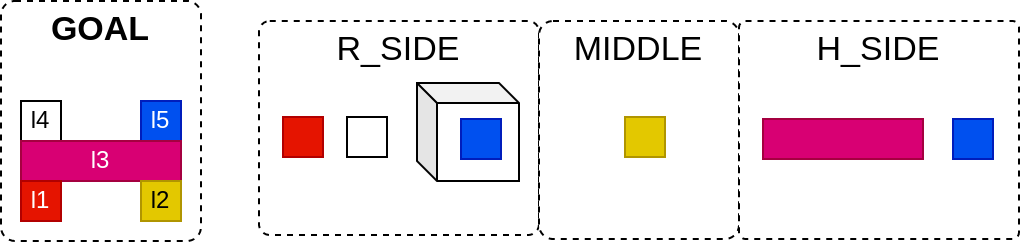
\includegraphics[width=\linewidth]{Chapter4/block_world_domain.png}
    \caption{An instance of the BlocksWorld domain. The ideal plan is strongly influenced by the human desired preferences. For the earliest end of the task, the human prevents using the box. A lazy human will only place the required pink bar from their side. A human in a hurry will concurrently place the yellow cube to place the pink bar at the earliest and be able to leave.}
    \label{fig:block_world_domain}
\end{figure}


    \subsection{Human Behavior and Erroneous Preferences Estimations}

To simulate human behavior, we consider and define human preferences that produce a human policy in the same manner as for the robot. The produced human policy makes the human always perform the best action regarding their defined preferences. The robot/planner does not have access to the human preferences but only to an estimation of them.

In order to evaluate the quality of the executed trace regarding the actual human preferences, we compare and rank every possible trace from the search graph, from best to worst. For legibility purposes, we normalize the ranks to obtain a score (H-score) s.t. the trace/plan with the lowest rank has a score of 0.0, while the highest rank corresponds to a score of 1.0. This score represents a quality indicator independent of the instance's size. 
Similarly, we can do the same and acquire the score regarding the robot's estimation of the preferences (R-score). 
Keep in mind that the R-score is an estimation of the actual H-score, and the robot acts in order to maximize its R-score, hoping to maximize the H-score as well.

However, the estimation of the human preferences can be more or less accurate, causing the robot's decisions to differ from what humans would have preferred. Once again, that's why making the robot compliant with human online decisions and actions gives the human more influence over the execution and helps to reach a high H-score even when the robot's estimation is incorrect.
Despite the robot trying to maximize its R-score, it's important to note that reaching a low R-score is fine as long as a high H-score is attained.

\begin{figure}
    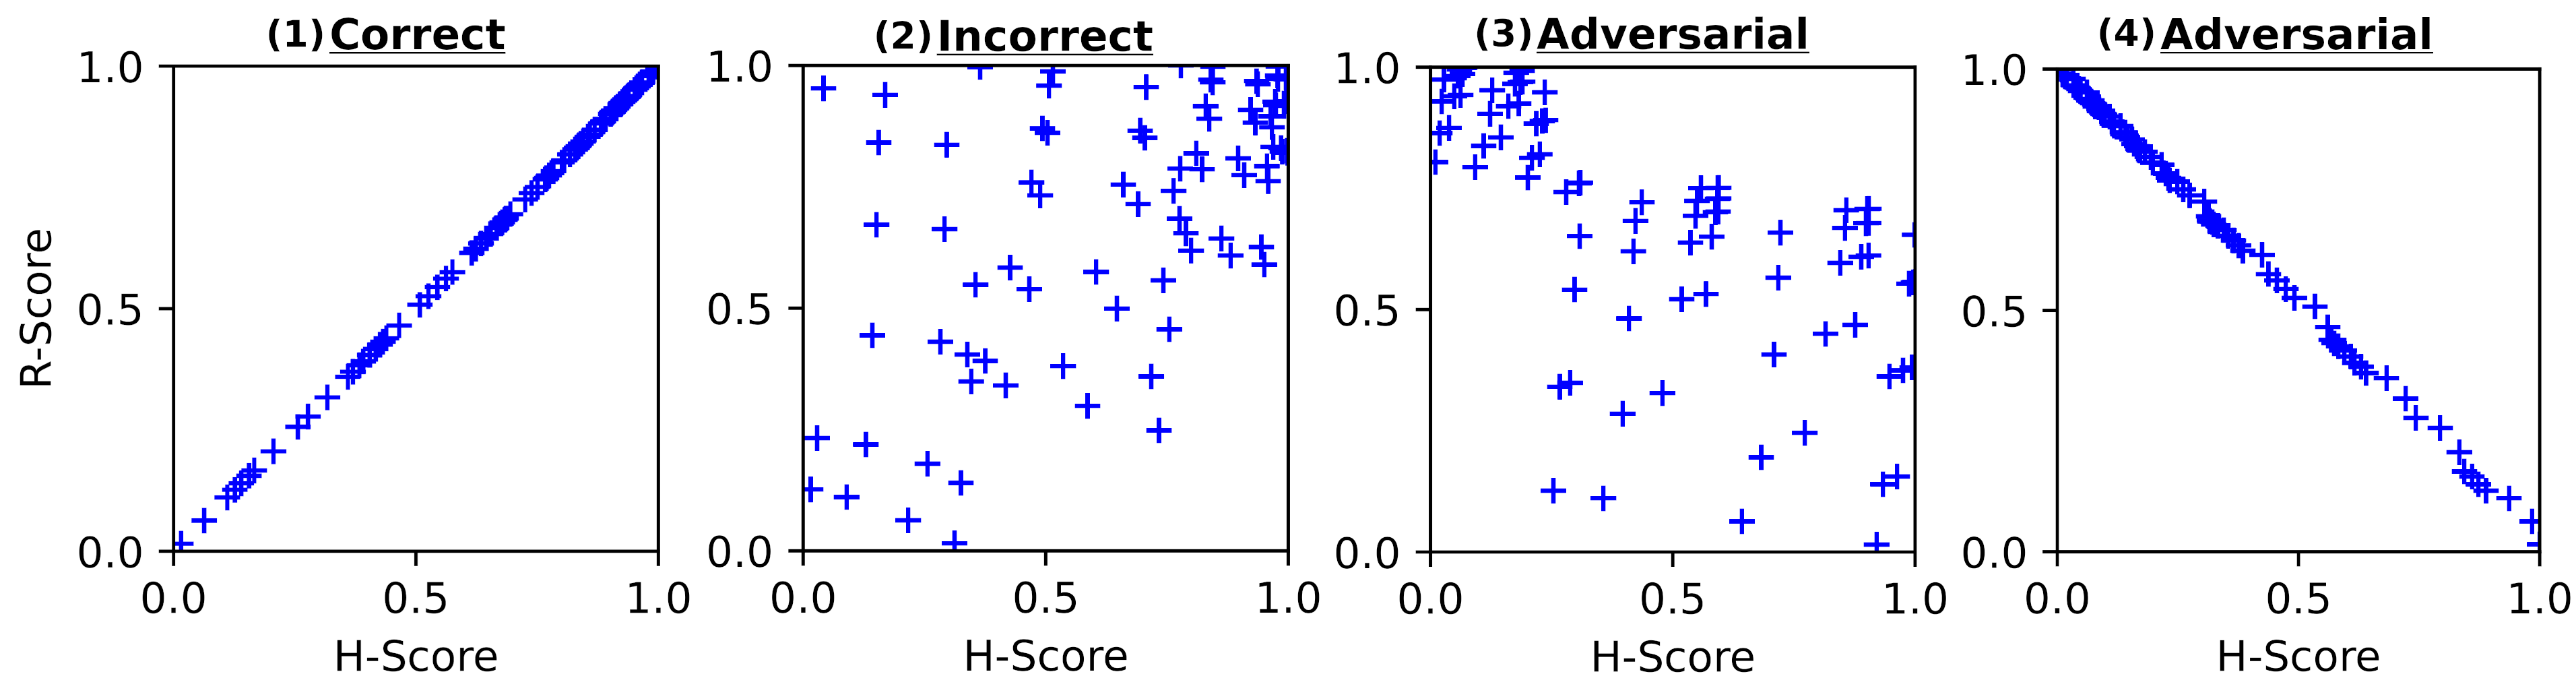
\includegraphics[width=\linewidth]{Chapter4/all_corr.png}
    \caption{
    Correlation between the H-score and R-score according to different robot estimations. Four pairs of human preferences and their estimation are considered. For each pair, all possible traces are plotted as blue crosses according to their H-score and R-score. \textit{(1)} show a correct estimation while the others show incorrect estimations. \textit{(3)} and \textit{(4)} depict \textit{adversarial} estimations.
    }
    \label{fig:corr}
\end{figure}

When solving the task, a pair of human preferences and their estimation creates a correlation between the possibly obtained H-scores and R-scores. Figure~\ref{fig:corr} depicts several possible correlations for the same task and the same search graph but different pairs of human preferences and their estimation. Each sub figure shows all possible traces as blue crosses according to their H-score and R-score. 
Let's consider the first case where the estimation is perfectly accurate (correct). Here, the robot's choices that maximize the R-score will necessarily maximize the H-score. Indeed, when considering the few top possible robot plans (crosses with near $1.0$ R-score), the human preferences are always well satisfied (near $1.0$). 
Let's now consider the second case where the robot estimation is incorrect. When considering again the few top possible robot plans a wide range of H-score can be reached (near $1.0$ as well as close to $0.0$). Thus, an incorrect estimation can satisfy the human preferences but not necessarily, leading to a wide range of H-score.
Eventually, consider the last two cases. Here, the lack of blue crosses in the top-right corners means that the H-score cannot be near $1.0$ while also having a high R-score. Consequently, when maximizing the R-score the robot will necessarily deteriorate the quality of the plan w.r.t. the H-score. We refer to these cases as \textit{adversarial} estimations since the robot involuntary goes against the human will. Such cases occur when the robot estimation is far from the actual preferences and intuitively goes against the latter, for instance, the robot trying to minimize the human effort while the human is actually trying to do as much as possible.  

    \subsection{Results}

\begin{figure}
    \centering
    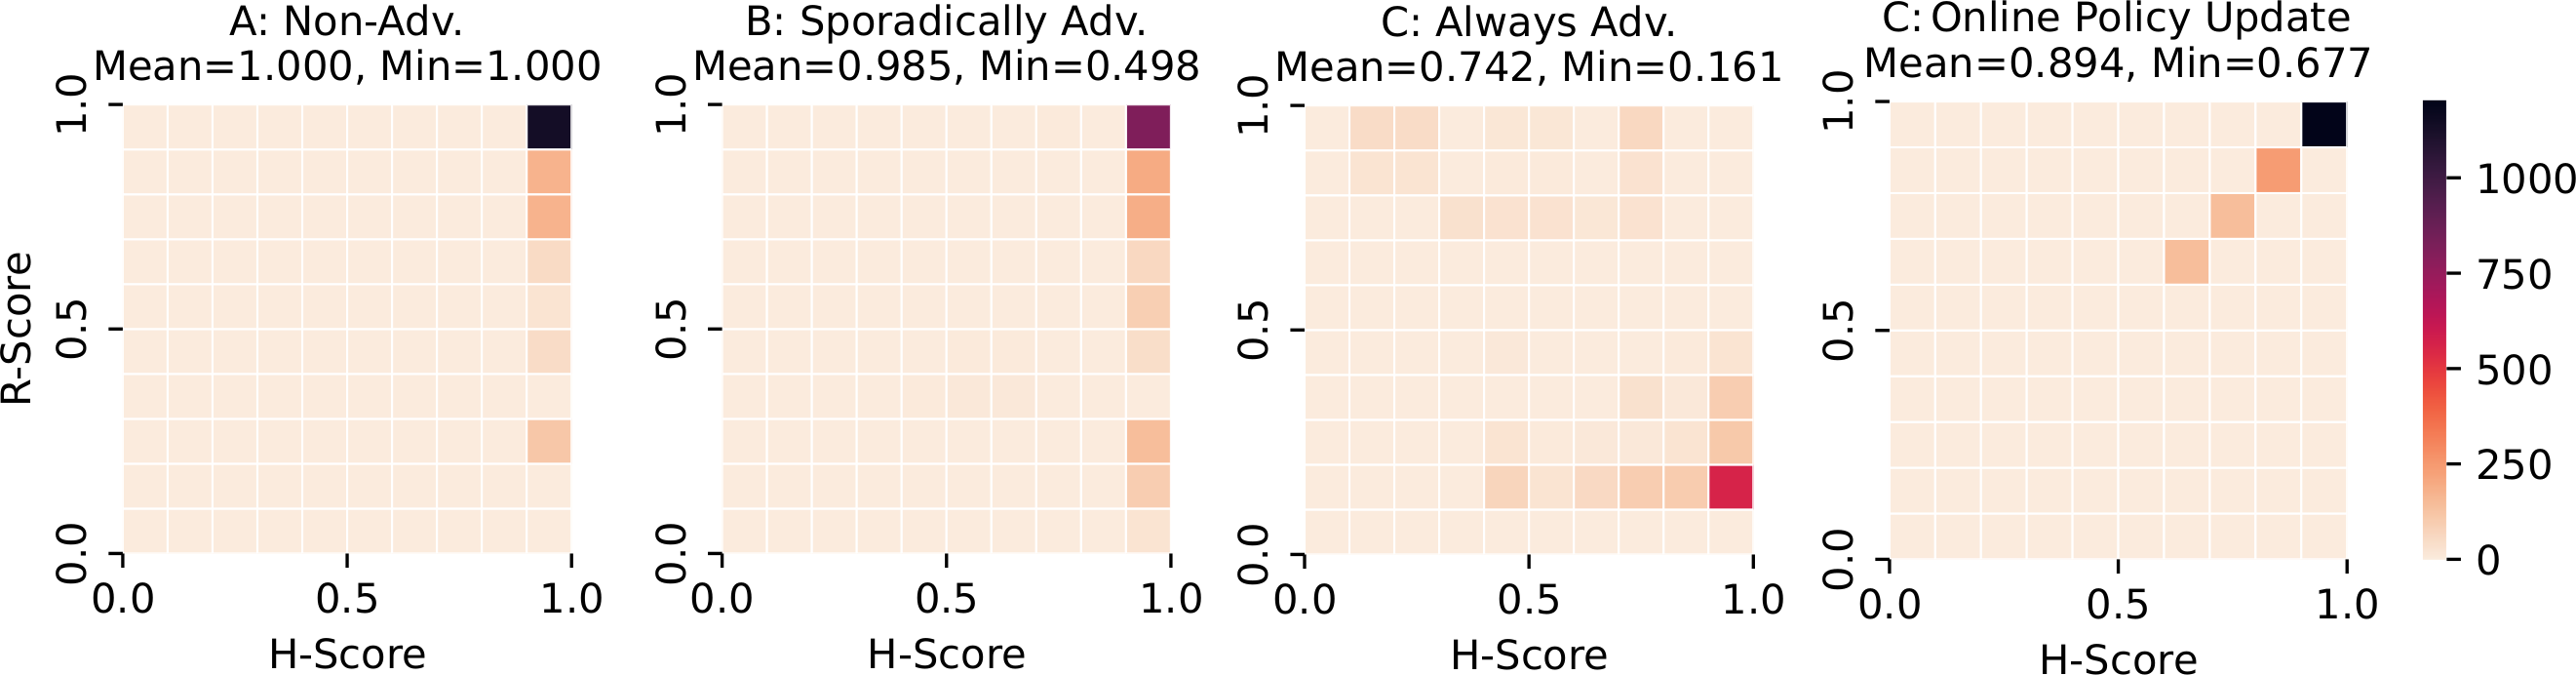
\includegraphics[width=\linewidth]{Chapter4/quant_results.png}
    \caption{
    R-scores and H-scores of the obtained executed plans after simulating the execution of the robot and the human policy generated by considering three problems and three sets of pairs of preferences/estimations. 
    The estimations in each set are (A) Never, (B) Sporadically, and (C) Always adversarial. On the right, the scores obtained using an enhanced human policy that can correct the robot's estimation online while using the set (C) is shown.
    }    
    \label{fig:heatmaps}
\end{figure}

For the simulations, we first generated three problems of the BlocksWorld domain with different initial states and shared tasks, and we produced their corresponding search graph for each. 
After that, we generated numerous pairs of human preferences and associated robot estimation, all those pairs are categorized into three distinct sets.

In Set~A, the estimations are mostly correct and close to the human preferences (case \textit{(1)} in figure~\ref{fig:corr}). Set~B includes incorrect estimations (case \textit{(2)} in figure~\ref{fig:corr}). And Set~C contains only adversarial estimations (cases \textit{(3)} and \textit{(4)} in figure~\ref{fig:corr}).
Then, for each preference-estimation pair and each problem, we generated the associated human and robot policies. Their execution was simulated symbolically using an execution automaton directly shaped upon the presented Model of Execution, and the obtained executed trace were retrieved.
The R-score and H-score of every obtained executed trace are shown as heatmaps for each distinct set of pairs in Figure~\ref{fig:heatmaps}. This will help us to highlight the benefits of using such an execution scheme.

In Set~A, the estimation of the robot is close to the real human preferences and is never adversarial. So, the robot policies (maximizing the R-score) should naturally lead to high H-scores, which we observed.
Some plans had an R-score lower than $1.0$, which shows that the estimation was imperfect. Nevertheless, the compliance to the human actions and the non-adversarial choices of the robot allows to always satisfy the maximal H-score of $1.0$, i.e., satisfy the human preferences everytime. 
With Set~B, the incorrect estimations induced some detrimental robot choices, preventing the human from always reaching a score of $1.0$. This is depicted by the minimal H-score of $0.498$ obtained. Nonetheless, the average H-score of $0.985$ indicates that the human preferences were overall largely met.
Set~C captures the worst possible estimations, inducing the robot to always make adversarial choices. This is depicted by the lower average H-score ($0.742$) and the very low minimal H-score obtained ($0.161$). 
However, we can notice that the average H-score is still high and that the R-score drops significantly. A low R-score means that the robot could not follow its policy correctly. Indeed, thanks to our model of execution, the robot complies with the human online decisions and purposely deviates from its ``optimal'' policy to let the human follow their own optimal policy. Eventually, the relatively high H-score obtained shows that the compliance is effective and compensates significantly (of course, not totally) for a very poor estimation of human preferences. 

Additionally, we can reasonably complement the human policy, which is based solely on preferences, with a \textit{rule}. Whenever the robot performs an action that significantly degrades the best reachable H-Score, the human reacts by correcting the robot estimation online.
The rightmost sub-figure in Figure~\ref{fig:heatmaps} shows the new scores obtained using the Set~C and the complemented human policy. 
We notice that correcting the estimation online avoids very low human scores (minimum of $0.677$) and increases significantly the average H-score compared with the original Set~C results (from $0.742$ to $0.894$). Hence, making the robot compliant with online preferences effectively improves the quality of the joint plan executed.

% \textbf{TODO: [Comparison with baseline ??? ... this lack was criticized... A simple baseline with Robot first? Should show that on correct is fine but then H-score is highly degraded... Should be a mirror case of our results However, must replicate results and create more... currently unclear if can replicate.]}

Overall, we can see that the compliant robot behavior regarding both online human actions and preferences benefits the collaboration thanks to the high human scores obtained.

Consider some counter-cases from social robotics (or HA collaborative planning). Assume a robot not giving the initiative to humans, always executing the best action it found. 
It is less acceptable and restricting for humans this way, even if the robot computed its best action by taking into account some social rules and estimated preferences. 
Unlike here, humans would appear compliant with the robots. 
In those cases, as evident from our simulation results in adversarial setups, the robot strongly impacts the solution H-score. Thus, wrong robot choices can significantly degrade the human scores. In some sense, being compliant and adjusting to online preferences can be seen as some social factor that robots should maximize, and our framework helps achieve that.

\section{Performances}


In this section, we discuss the computational performances of our approach and provide some empirical measurements. 

Our approach is based on exploring every decision the human is likely to make and every possible robot concurrent and compliant actions to those decisions. 
This offline search produces a \acrfull{dag}, which captures all possible courses of action. Then, from this graph, we can easily extract online the optimal robot policy to adapt to and to satisfy the human preferences. However, this exhaustive approach does not scale since the more complex and lengthy the task is, the more possible coordinations and courses of action exist, and the longer it takes to produce the graph. Despite this existing combinatory explosion, I would like to discuss and explain why our approach is still relevant.

Two cases can be identified. The first one is in an industrial setup, and the other is in a household environment. Industrial tasks can be complex, constrained, and where mistakes can have heavy consequences. However, household tasks are usually simpler, shorter, and have fewer constraints and consequences. Due to the nature of industrial tasks, there is usually a known pre-defined protocol or plan to solve the task. The human is also in a working mental state, being more focused and willing to collaborate and accept robot decisions. In such setups, it is more acceptable for the robot to produce a joint plan and negotiate with the human to accept and follow it without anticipating every possible human decision, significantly reducing the planning algorithm's complexity.
On the other hand, when considering household tasks, which is more our focus in this work, we want to preserve the human's latitude of choice as much as possible to allow them to change their mind, be distracted, or impose their choice. For this reason, it is adequate to run an exhaustive search and account for every possibility. 

Overall Human-Robot Collaboration scenarios never require long plans, especially household tasks, and are often limited to about 20 actions per agent. For such length, our exhaustive approach performs efficiently. Our approach takes about $0.40s$ to produce the \acrshort{dag} for the BlocksWorld task described in chapter~\ref{chap:6}. This graph comprises $700$ nodes and $6$ leaves, corresponding to $6839430$ different possible plans of length $19.77 \pm 1.59$ steps. With millions of plans, we explore sufficient possibilities to address such collaboration problems correctly. Moreover, it takes only $0.02s$ to extract the robot's policy from the produced graph. 

% \textbf{TODO: Try to add more numbers, about the task of Chapter 4 with box, and about more complex and long tasks}


\section{Discussion and Limitations}


This section discusses a few limitations of the proposed approach and possible future works to overcome them. 

First, in order to explore relevant courses of action, we assume a step-based progression toward the goal. Hence, we assume that the human and the robot must synchronize together after every action. This can work efficiently as long as we assume that all actions have roughly the same durations. However, in practice, this is never precisely the case, and one agent must wait for the other at every step. Since the robot tends to be slower, the human might have to often wait for the robot during the collaboration with these assumptions. To be implemented on a real robot, this approach requires an additional execution scheme supervising the plan execution. In specific situations, this scheme could skip one synchronization and synchronize after the next step. Such a scheme could allow humans to perform more actions than robots before synchronizing, thus promoting smooth and flexible execution.

Speaking of execution, the results presented in this chapter have only been simulated symbolically, without durative actions nor real human decisions. The next two chapters (\ref{chap:5} and \ref{chap:6}) present a user study conducted on an interactive simulator where participants collaborated with a simulated robot executing the produced policy. To do so, we created an execution scheme that supervises the execution of the robot policy with agent synchronizations. This scheme is directly based on the model of execution presented in fig.~\ref{fig:complete_model_exec}. Thus, it relies on the steps and does not provide the flexible execution mentioned just above. 

Additionally, in the proposed model of execution, the robot always gives the initiative to the human. We show that this decision makes the collaboration robust to erroneous human preference estimations and, thus, is beneficial. However, sometimes, it could be relevant for the robot to switch from follower to leader intelligently. Indeed, currently, even when there are no possible conflicts between agents' actions, the robot waits for the human to start acting to begin. Such synchronization is not really necessary, so the robot could start acting directly to solve the task faster. 

Eventually, the plan evaluation is limited. For now, plan selection relies on the estimated human preferences, which are a list of metrics to maximize or minimize in the priority order given by the list. This means that there is no balance between the metrics so, depending on the ordering, a plan of length $N$ where the robot is never intrusive and always compliant could be rejected against a plan of length $N-1$ where the robot is intrusive twice and never compliant. 
However, in our examples, we tend to explore numerous very similar possible plans. Thus, there are always several possible plans with the same top-priority metric value, e.g., plan length, and the ordering will help select the best plan that satisfies the other listed metrics.   

\section{Conclusion}

We addressed the complex challenge of concurrent task planning for a shared goal in the context of human-robot collaboration, acknowledging the inherent need for autonomy in humans' choices of `what' and `how' aspects during task execution. 

Based on studies about joint action, we formulate an execution model and present a new human-aware task planner designed to accommodate the uncontrollability factor inherent in human agents while employing this execution model leveraging social signals to facilitate the exploration of human-robot joint actions and smooth execution. 
We also propose a plan evaluation and selection based on estimations of the human inner preferences.
As a result, the planner produces the behavioral policy for a robot that complies with online human decisions and their (online) provided estimated preferences, 
ensuring it solves the task, satisfies at best the estimated human preferences, and allows smooth and sound execution of concurrent joint action.

We provide a detailed account of the novel planning process and joint action model. We demonstrated its effectiveness through symbolically simulated BlocksWorld scenarios and how our model makes the robot robust to erroneous preference estimations.

Additionally, as mentioned in the previous section, we implemented an interactive simulator in which a real human can collaborate with a simulated robot running the generated policies. We used this simulator to conduct a user study to validate our approach with real humans. This simulator and study are described in the next two chapters.  
